% Beamer presentation rewritten from provided LaTeX content
\documentclass[aspectratio=169]{beamer}

% Theme suggestion (can be changed)
\usetheme{Copenhagen}

\setbeamertemplate{navigation symbols}{} % To remove the navigation symbols from the bottom of all slides uncomment this line
\setbeamertemplate{footline}[frame number] % To replace the footer line in all slides with a simple slide count uncomment this line

% Set color
\definecolor{UBCblue}{rgb}{0.04706, 0.13725, 0.26667} % UBC Blue (primary)
\usecolortheme[named=UBCblue]{structure}

% TikZ and libraries
\usepackage{tikz}
\usetikzlibrary{arrows.meta, positioning}

\usepackage{subfig}
% \usepackage{subcaption}
\usepackage[justification=centering]{caption}
\usepackage{booktabs}
\usepackage{array}

% Title information
\title{The Effect of Climate Change on Landslides}
\author{Nathasya Christien}
\date{\textit{Based on Crozier's paper}}

\begin{document}

\frame{\titlepage}

% Traditional view slide
\begin{frame}{Today's Relevancy: Recent news from Indonesia}

\begin{columns}[c]
    \column{.6\textwidth}
    \begin{figure}[H] % H
    \centering
    \includegraphics[height=5.75cm]{fig/antara.png}
    \captionsetup{justification=centering, margin=0.5cm}
    \captionsetup{justification=centering, margin=0.5cm, skip=2pt}
    \tiny
    \caption*{Landslide disaster in North Sumatra (December 6, 2025) \\Source: Antara News, 2025}
    \end{figure}

    
    \column{.4\textwidth}
    \begin{itemize}
        \item Cyclone-induced floods and landslides impact North Sumatra. \pause
        \item It marks the deadliest disaster since 2018 earthquake and tsunami in Sulawesi.
    \end{itemize}
\end{columns}
\end{frame}

\begin{frame}{Today's Relevancy: Recent news from Indonesia}
    \begin{columns}[c]
    \column{.5\textwidth}
    \begin{figure}[H] % H
    \centering
    \includegraphics[height=5.0cm]{fig/batangtoroe.png}
    \captionsetup{justification=centering, margin=0.5cm}
    \captionsetup{justification=centering, margin=0.5cm, skip=2pt}
    \tiny
    \caption*{Deforestation and forest degradation around Batang Toru from Google Earth Imagery \\ Source: The Conversation, 2025}
    \end{figure}

    
    \column{.5\textwidth}
    \begin{itemize}
        \item Public has pointed out how this disaster is also human-induced. \pause
        \item Example in Batang Toru: Around 1,550 hectares of the forests in the area have lost their vegetation cover.
    \end{itemize}
\end{columns}
\end{frame}

\begin{frame}{Influential Papers on This Topic}
    \begin{figure}[H] % H
    \centering
    \includegraphics[height=6.5cm]{fig/influential_papers.png}
    \captionsetup{justification=centering, margin=0.5cm}
    \captionsetup{justification=centering, margin=0.5cm, skip=2pt}
    \tiny
    \caption*{Most cited papers as seen in Mendeley search engine}
    \end{figure}
\end{frame}

\begin{frame}{Physics of Slope Stability}
    \begin{definition}
        Factor-of-safety is expressed as
        \[ FS = \frac{s}{\tau} \]
        with shear strength $s$ and shear stress $\tau$ on a potential surface of rupture. \pause
        In simpler terms,
        \[ FS = \frac{\text{resisting force}}{\text{driving force}}.\]
    \end{definition}

    \pause

    \textbf{Interpretation:}
    \begin{itemize}
        \item If $FS > 1$, slope is stable.
        \item If $FS = 1$, slope is at point of failure.
        \item If $FS < 1$, slope will slide.
    \end{itemize}
\end{frame}

\begin{frame}{Physics of Slope Stability}
    \begin{block}{}
    \begin{columns}[c]
    \column{.4\textwidth}
    Let
    \begin{itemize}
        \item $c$ : cohesion
        \item $\gamma$ : bulk density
        \item $z$ : vertical depth
        \item $\beta$ : slope angle
        \item $u$ : porewater pressure
        \item $\phi$ : angle of internal friction
    \end{itemize}
    
    \column{.5\textwidth}
    We expand the terms, such that the resisting force becomes
    \[ s = c + (\gamma z \cos^2{\beta} - u) \tan{\phi} \]
    and driving force becomes
    \[ \tau = \gamma z \sin{\beta} \cos{\beta}. \]
    \end{columns}
    \end{block}

    \pause

    \textbf{How heavy rainfall reduces shear strength:}
    \begin{itemize}
        \item Increases water weight
        \item Increases porewater pressure
        \item Reduces soil suction
        \item Weathering cycles
    \end{itemize}
    
\end{frame}

\begin{frame}{Physics of Slope Stability}
\footnotesize
\centering
\textbf{Slope stability responses to climatic factors change}

\vspace{0.4cm}

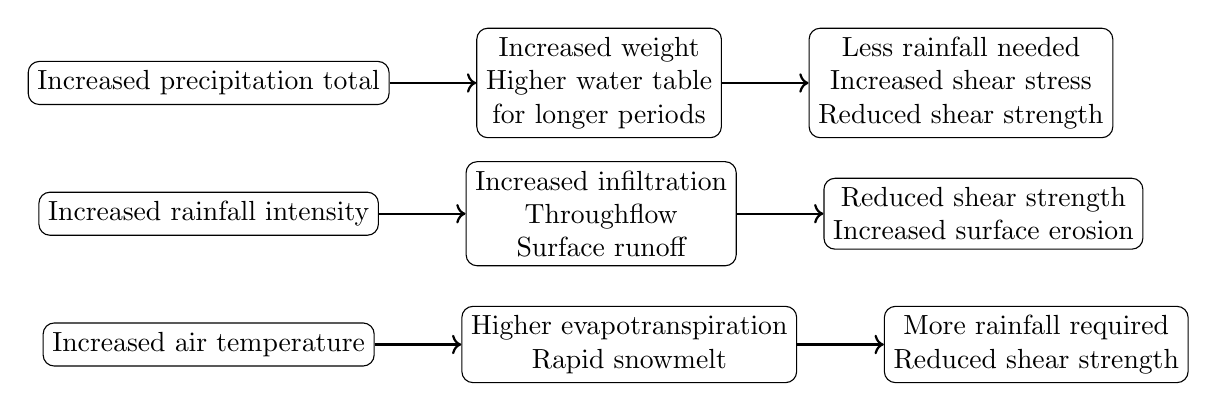
\begin{tikzpicture}[
    node distance=1.1cm,
    every node/.style={draw, rounded corners, align=center},
    arrow/.style={->, thick}
]

% Row 1
\node (c1) {Increased precipitation total};
\node (p1) [right=of c1] {Increased weight\\ Higher water table\\ for longer periods};
\node (e1) [right=of p1] {Less rainfall needed\\ Increased shear stress\\ Reduced shear strength};

\draw[arrow] (c1) -- (p1);
\draw[arrow] (p1) -- (e1);

% Row 2
\node (c2) [below=of c1] {Increased rainfall intensity};
\node (p2) [right=of c2] {Increased infiltration\\ Throughflow\\ Surface runoff};
\node (e2) [right=of p2] {Reduced shear strength\\ Increased surface erosion};

\draw[arrow] (c2) -- (p2);
\draw[arrow] (p2) -- (e2);

% Row 3
\node (c3) [below=of c2] {Increased air temperature};
\node (p3) [right=of c3] {Higher evapotranspiration\\ Rapid snowmelt};
\node (e3) [right=of p3] {More rainfall required\\ Reduced shear strength};

\draw[arrow] (c3) -- (p3);
\draw[arrow] (p3) -- (e3);
\end{tikzpicture}
\end{frame}

\begin{frame}{Physics of Slope Stability}
\footnotesize
\centering
\textbf{Slope stability responses to climatic factors change}

\vspace{0.4cm}

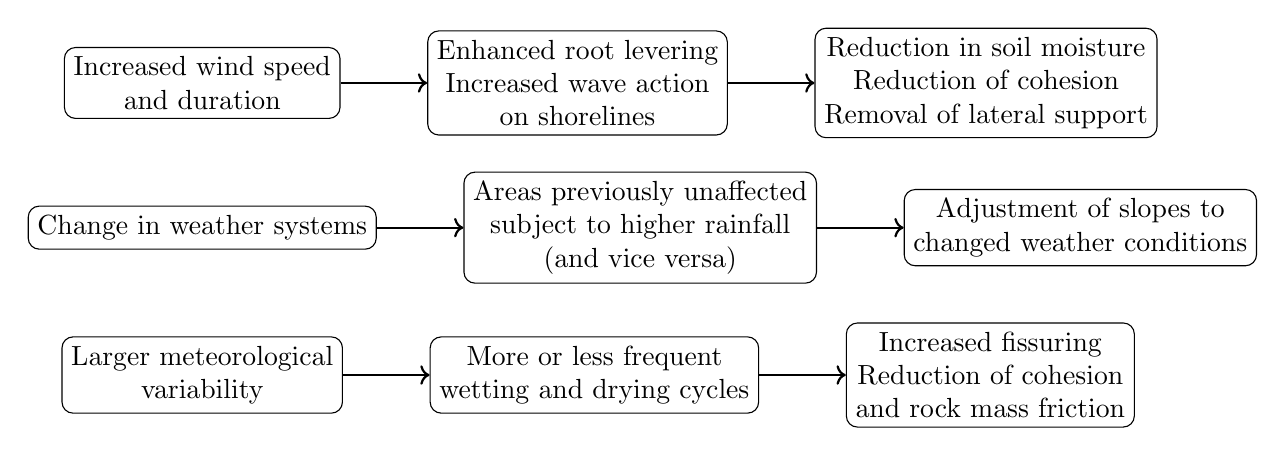
\begin{tikzpicture}[
    node distance=1.1cm,
    every node/.style={draw, rounded corners, align=center},
    arrow/.style={->, thick}
]

% Row 4
\node (c4) {Increased wind speed\\ and duration};
\node (p4) [right=of c4] {Enhanced root levering\\ Increased wave action\\ on shorelines};
\node (e4) [right=of p4] {Reduction in soil moisture\\ Reduction of cohesion\\ Removal of lateral support};

\draw[arrow] (c4) -- (p4);
\draw[arrow] (p4) -- (e4);

% Row 5
\node (c5) [below=of c4] {Change in weather systems};
\node (p5) [right=of c5] {Areas previously unaffected\\ subject to higher rainfall\\ (and vice versa)};
\node (e5) [right=of p5] {Adjustment of slopes to\\ changed weather conditions};

\draw[arrow] (c5) -- (p5);
\draw[arrow] (p5) -- (e5);

% Row 6
\node (c6) [below=of c5] {Larger meteorological\\ variability};
\node (p6) [right=of c6] {More or less frequent\\ wetting and drying cycles};
\node (e6) [right=of p6] {Increased fissuring\\ Reduction of cohesion\\ and rock mass friction};

\draw[arrow] (c6) -- (p6);
\draw[arrow] (p6) -- (e6);

\end{tikzpicture}
\end{frame}

\begin{frame}{Local Slope Hydrology Dominates Climate Change Impact}

\textbf{Climate signals are strongly filtered by local slope conditions:}

\begin{itemize}
    \item Degree of existing inherent instability
    \item Landslide type (shallow vs deep)
    \item First-time failure vs reactivation
\end{itemize} \pause

\vspace{0.3cm}

\textbf{Key physical constraint (often overlooked):}
\begin{block}{}
Failure requires water to \emph{accumulate} in the slope:
\[
\text{Infiltration rate} > \text{Drainage rate}
\]
\end{block} \pause

\vspace{0.2cm}

\textbf{Implication:}
Soil \emph{infiltration capacity} governs how much rainfall actually enters the slope.
\pause
\vspace{0.3cm}

\textbf{Observed example in Hong Kong (So, 1971):}
\begin{itemize}
    \item $\sim$702 landslides triggered by $\sim$400 mm rainfall in one day
    \item 35\% occurred in forested areas, despite covering only 8\% of the affected region
\end{itemize}

\end{frame}


\begin{frame}{Climate-Landslide Model Results: Antecedent water status model}
    \begin{columns}[c]
    \column{.65\textwidth}
    \begin{figure}[H] % H
    \centering
    \includegraphics[height=5.5cm]{fig/awsm.png}
    \captionsetup{justification=centering, margin=0.5cm}
    \captionsetup{justification=centering, margin=0.5cm, skip=2pt}
    \tiny
    \caption*{Author's model applied in Wellington City, New Zealand}
    \end{figure}

    \column{.35\textwidth}
    \begin{itemize}
        \item The model empirically estimates the amount of event rainfall required to initiate landslides for the next 24 hour periods. \pause
        \item From IPCC downscaled prediction, we expect 8\% increase of a 100-year daily rainfall.
        \end{itemize}
    \end{columns}
\end{frame}

\begin{frame}{Climate-Landslide Model Results: Antecedent water status model}
    \begin{columns}[c]
    \column{.65\textwidth}
    \begin{figure}[H] % H
    \centering
    \includegraphics[height=5.5cm]{fig/awsm.png}
    \captionsetup{justification=centering, margin=0.5cm}
    \captionsetup{justification=centering, margin=0.5cm, skip=2pt}
    \tiny
    \caption*{Author's model applied in Wellington City, New Zealand}
    \end{figure}

    \column{.35\textwidth}
    \begin{itemize}
        \item With climate change scenario, two extra days of landslides could occur. \pause
        \item Limitation: Downscaled rainfall data had too many uncertainties. 
    \end{itemize}
    \end{columns}
\end{frame}

\begin{frame}{Climate-Landslide Model: Regional empirical approach}
    \begin{columns}[c]
    \column{.6\textwidth}
    \begin{figure}[H] % H
    \centering
    \includegraphics[height=5.5cm]{fig/empirical_model.png}
    \captionsetup{justification=centering, margin=0.5cm}
    \captionsetup{justification=centering, margin=0.5cm, skip=2pt}
    \tiny
    \caption*{The frequency of landslide events ($y$) vs mean annual rainfall ($x$) around New Zealand (Hicks, 1995)}
    \end{figure}

    \column{.4\textwidth}
    \begin{itemize}
        \item Collected from 12 different catchments in New Zealand. \pause
        \item The equation for the trend is
        \[y = 3009 x^{-8939}, s= 1.0\]
        with $s$ as standard error of the estimate $y$. \pause
        \item An 8\% rise in annual rainfall (from 1000 mm) $\rightarrow$ number of events from 16 to 20 over a 100 year period.
    \end{itemize}
    \end{columns}
\end{frame}

\begin{frame}{Climate-Landslide Model: Regional empirical approach}
    \begin{columns}[c]
    \column{.6\textwidth}
    \begin{figure}[H] % H
    \centering
    \includegraphics[height=5.5cm]{fig/empirical_model.png}
    \captionsetup{justification=centering, margin=0.5cm}
    \captionsetup{justification=centering, margin=0.5cm, skip=2pt}
    \tiny
    \caption*{The frequency of landslide events ($y$) vs mean annual rainfall ($x$) around New Zealand (Hicks, 1995)}
    \end{figure}

    \column{.4\textwidth}
    \begin{itemize}
        \item Uncertainty factors:
        \begin{itemize}
            \item Predicted low and high estimates of mean precipitation is too large. \pause
            \item The standard error is still large. \pause
            \item Could not capture the full range of terrain, material, and vegetation throughout the country.
        \end{itemize}
    \end{itemize}
    \end{columns}
\end{frame}

\begin{frame}{The Human Factor}
\begin{columns}[c]
    \column{.5\textwidth}
    \begin{figure}[H] % H
    \centering
    \includegraphics[height=5.5cm]{fig/forest_vs_pasture.png}
    \captionsetup{justification=centering, margin=0.5cm}
    \captionsetup{justification=centering, margin=0.5cm, skip=2pt}
    \tiny
    \caption*{Contrast in landslide distribution between forested and pasture slopes in Manawatu, New Zealand (Feb 2004)}
    \end{figure}

    \column{.5\textwidth}
    \begin{itemize}
        \item The impact of human activity on landsliding can be seen with greater certainty than that of future climate change. \pause
        \item Examples from New Zealand:
        \begin{itemize}
            \item Forest converted to pasture increases landslide probability by 3×. \pause
            \item Sedimentation rate increased by 5× after European farming practices commenced in New Zealand. \pause
            \item Deforestation increases runoff 28\%, whereas climate-change-driven runoff increase is ~15\%. \pause
        \end{itemize}
        \end{itemize}
\end{columns}
\end{frame}

\begin{frame}{The Human Factor}
\begin{columns}[c]
    \column{.5\textwidth}
    \begin{figure}[H] % H
    \centering
    \includegraphics[height=5.5cm]{fig/forest_vs_pasture.png}
    \captionsetup{justification=centering, margin=0.5cm}
    \captionsetup{justification=centering, margin=0.5cm, skip=2pt}
    \tiny
    \caption*{Contrast in landslide distribution between forested and pasture slopes in Manawatu, New Zealand (Feb 2004)}
    \end{figure}

    \column{.5\textwidth}
    \textbf{About increase of hazard:}
    \begin{itemize}
        \item Comparing 2004 to 1900, the world's population has increased 4$\times$, while economic activity has increased by 40$\times$.
        \item More people increases landslide losses, but human alteration of slopes increases landslide occurrence itself.
    \end{itemize}
\end{columns}
\end{frame}

\begin{frame}{Take-Home Messages}
    \begin{enumerate}
        \item Climate change can increase landslides. \pause
        \item However, prediction is extremely uncertain. \pause
        \item Human land-use changes often dominate. \pause
        \item We need collaboration between climate and slope-stability modellers.
    \end{enumerate}
\end{frame}

\end{document}
